%\documentclass{standalone}
%\usepackage{tikz}

%\begin{document}

%\begin{minipage}{0.55\textwidth}
%	\centering
	\def\rowperm{{0, 1, 2, 3, 4, 5, 6}}
	%\def\colperm{{0, 1, 2, 3, 4, 5, 6}}
	\def\colperm{{0, 1, 2, 3, 4, 5, 6}}
	\scalebox{0.7}{\begin{tikzpicture}
		\foreach \x in {0,1}
		\fill[gray] (\colperm[\x]-1,6) rectangle (\colperm[\x],7);
		\foreach \y in {0,1,2,3,4}  
			\foreach \x in {0,1,2}
				\fill[gray] (\colperm[\x]-1+\y,5-\y) rectangle (\colperm[\x]+\y,6-\y);   
		\foreach \x in {0,1}
			\fill[gray] (\colperm[5+\x]-1,0) rectangle (\colperm[5+\x],1); 	
		\draw[step=1cm,black,very thin] (-1,-0) grid (6,7);
		\node at (6.4,3.5) {\fontsize{25}{25}\selectfont {*}};
		\end{tikzpicture}}
	%\hspace{0.1cm}
	\scalebox{0.7}{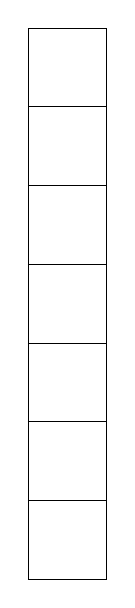
\begin{tikzpicture}
		\draw[step=1cm,black,very thin] (8,-0) grid (9,7);
	\end{tikzpicture}}

%\end{minipage}
%\end{document}
